\documentclass[12pt]{report}
\usepackage[utf8]{inputenc}
\usepackage{graphicx}
\graphicspath{ {images/} }

\usepackage[a4paper,width=150mm,top=25mm,bottom=25mm]{geometry}
\usepackage{fancyhdr}
\pagestyle{fancy}
\fancyhead[RO]{CH. \thechapter}

\usepackage{caption}
\usepackage{subcaption}

\usepackage[backend=biber]{biblatex} 
\addbibresource{references.bib}

\usepackage{setspace}
\doublespacing

\begin{document}

%%%%%%%%%%%%%%%%%%%%%%% Begin Title Page %%%%%%%%%%%%%%%%%%%%%%%%%%
\begin{titlepage}
    \begin{center}
    
        \vspace*{2cm}
        
        \LARGE
        Optimal Control: A Comparison in Performance of Reinforcement Learning versus Model Predictive Control \\
        
        \vspace{1cm}
        
        \normalsize by \\
        
        \vspace{1cm}
        
        \large Rui Nian \\
        
        \vspace{3.5cm}
        
        A thesis submitted in partial fulfillment of the requirements for the degree of \\
        \vspace{1cm}
        Masters of Science in Process Control \\
        
        \vspace{4cm}
        
        Department of Chemical and Materials Engineering \\
        University of Alberta \\
        
        \vspace{1.5cm}
        
        \textcopyright \hspace{1mm} Rui Nian, 2019 \\
        

    \end{center}
\end{titlepage}
%%%%%%%%%%%%%%%%%%%%%%% End Title Page %%%%%%%%%%%%%%%%%%%%%%%%%%



%%%%%%%%%%%%%%%%%%%%%%%%%%%% Begin Main Document %%%%%%%%%%%%%%%%%%%%%%%%%%%%%%%%
\chapter*{Abstract}

\tableofcontents
\listoffigures
\listoftables

\chapter*{Acknowledgements}

\chapter*{Nomenclature}

\chapter{Introduction}
\section{Introduction to the Optimal Control Problem}

\section{Motivation and Challenges}

\section{Thesis Outline and Contributions}


\chapter{Markov Decision Processes}
\section{Markov Decision Processes}

\section{Semi Markov Decision Processes}

\section{Partially Observable Markov Decision Processes}


\chapter{Reinforcement Learning}
Reinforcement learning is a goal-directed learning algorithm which continually improves its own performance through interactions with the environment \cite{sutton}. The main objectives of reinforcement learning are to identify hidden structures within the environment and to find the optimal policy (i.e., optimal input trajectory) through guidance from an internal scalar reward (feedback). Two distinct characteristics that deviate reinforcement learning from other methods are its trial \& error search to find the optimal policy, and its ability to identify delayed reward signals. Modern reinforcement learning methods combines principles of optimal control and learning methods together to solve for the optimal control trajectory in an environment.  In this chapter, fundamental reinforcement learning concepts are first introduced.  Then, tabular based methods will be shown.  However, due to the "curse of dimensionality" of high dimensional problems, tabular based approaches fail to bear fruit.  To overcome these issues, deep neural networks will be used as function approximation, and deep reinforcement learning will be introduced.


\section{Introduction to Reinforcement Learning}

In general terms, reinforcement learning is simply the learning an agent experiences through interactions with the environment.  For added intuition, Figure \ref{fig: simple_rl} shows the generic information flow of reinforcement learning. First, the agent observes some states, $x_t \in \mathbb{X}$, from the environment (some states may be unobservable).  Given $x_t$, the agent performs some actions, $u_t \in \mathbb{U}$ and receives a scalar reward signal, $r_{t+1} \in \mathbb{R}$.  Finally, the environment will transition to a new state, $x_{t+1}$, given probability $P(x_{t+1}, r_{t+1} | x, u)$.

\begin{figure}[h]
    \centering
    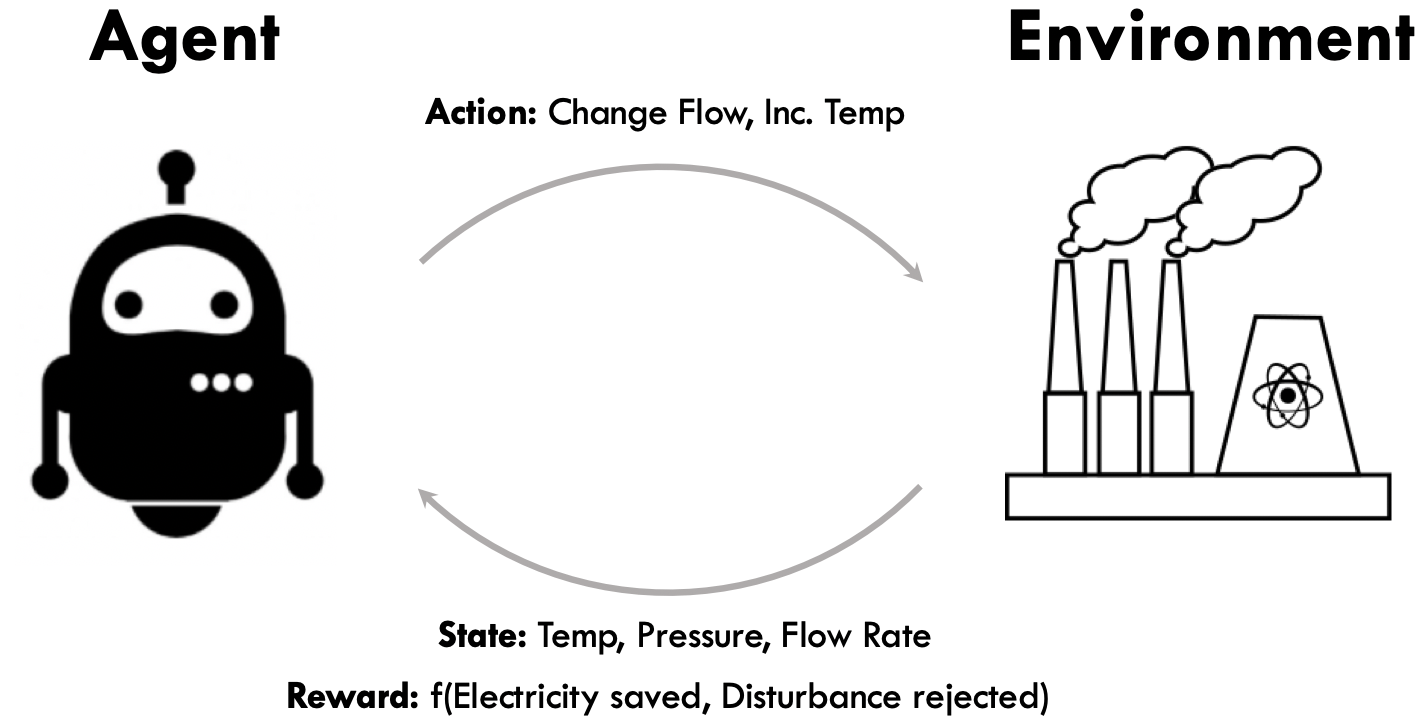
\includegraphics[scale=0.5]{images/RL.png}
    \caption{Basic setup of reinforcement learning where an agent interacts with the environment}
    \label{fig: simple_rl}

\end{figure}

Reinforcement learning consists of the following four elements:

\begin{itemize}
    \item Policy, $\pi$
    \item Reward, $R$
    \item Value Function, $V(s)$
    \item Model (optional), $\dot{x} = Ax + Bu$
\end{itemize}

The policy, $\pi$, of reinforcement learning is a direct mapping from $X \rightarrow U$.  To find the optimal policy, $\pi^*$, the agent is guided by an immediate scalar reward for each interaction (also called \textit{episode}). Policies resulting in higher rewards are more likely to be followed in the future, \textit{mutatis mutandis}.  However, reinforcement learning is concerned with the long term success rather than immediate pleasure. Often times, long term success require short term sacrifice.  Thus, the value function, $V^{\pi}(s)$, is used to describe the long term expected reward under each policy.  Initially, the value function for each state is initialized at zero.  After each episode, the value function will be updated to reflect the new knowledge obtained from the last episode through Equation \ref{eq: value_function}.

\begin{equation}
    \centering
    V(x_t) \leftarrow V(x_t) + \alpha [V(x_{t + 1}) - V(x_t)]
    \label{eq: value_function}
\end{equation}

In Equation \ref{eq: value_function}, $\alpha$ represents the step-size parameter.  That is, how big each update step should be.  Once convergence is achieved for $V(x_t)$, the optimal policy can be described by Equation \ref{eq: opt_policy}.  

\begin{equation}
    \centering
    \pi^*(x) = \argmax_u q_{\pi}(x, u), \; \forall x 
    \label{eq: opt_policy}
\end{equation}

Lastly, reinforcement learning \textit{can} consist of a model. Such cases are called \textit{model-based} reinforcement learning.  The model will be used for planning, and is a way for the agent to plan a control trajectory before they are experienced.  Contrarily, \textit{model-free} reinforcement learning learns \textit{explicitly} through interactions with the environment.

One key topic of reinforcement learning is: \textbf{exploration} vs. \textbf{exploitation}.  At first, the agent must explore to learn the state space, $\mathcal{X}$.  But the agent must know \textit{when} to stop exploring, and start exploiting (i.e., start taking advantage of what is known).  If the agent explores too much, lots of value is lost.  However, if the agent does not explore enough, the current policy may not be optimal and more value is lost long term.  Exploration vs. exploitation is one of the most important topics today in reinforcement learning, and the time to switch from exploration to exploitation will vary between problems.  In control theory, exploration vs. exploitation is known as the conflict between identification (or estimation) and control \cite{explorevexploitcontrol}.  

Another important distinction between different reinforcement learning algorithms is \textbf{on-policy} vs. \textbf{off-policy}.  On-policy methods select actions that maximizes reward given the current knowledge of the agent.  Subsequently, off-policy methods perform exploratory actions for a chance that the explored action offers superior returns to the current best known action.

\subsection{Reinforcement Learning Basics}

Reinforcement learning takes its roots from the \textit{k-armed bandit problem} that has been studied in engineering, psychology, and statistics.  Originally, the problem disregarded state information, and only worried about the optimal actions for solving \textit{one} specific situation \cite{thompson1, thompson2, robbins, bellman_bandit}.  As a natural extension, Barto, Sutton and Brouwer extended the idea to multi-situation systems \cite{bartosuttonbrouwer} through associative search, also known as \textit{contextual bandits}. The main objective of this algorithm was to find an optimal policy for each situation, $\pi^*(x)$.  However, it only concerns the immediate rewards and not the long term consequences.  Reinforcement learning was then developed to find the optimal policy for each situation and the onward trajectory there-forth.  

\subsubsection{\textit{k}-armed Bandit}

The \textit{k}-armed bandit is the fundamentals to understanding modern reinforcement learning.  Here, an agent is present and must choose action $u$ from $\mathbb{U}$, where $\mathbb{U}$ has $k$ choices.  After each action, a scalar reward from a stationary distribution will be returned to the agent as feedback.  The objective of the agent is to ultimately maximize reward over $N$ steps.  For each action, there is an expected reward called \textit{value}, given by Equation \ref{eq: value}.

\begin{equation}
    \centering
    q_*(a) = \mathbb{E}[R_t | A_t = a]
    \label{eq: value}
\end{equation}

The real value is unknown, however, an estimation can be computed and is denoted as $Q_t(a)$.  Given all $Q_t(a)$ is maintained, at any time, one $Q_t(a)$ will be greater than all others.  Picking the action that corresponds to the maximum $Q_t(a)$ is known as \textit{greedy}, and the agent is said to be \textit{exploiting}.  If a non-maximum action is picked, the agent is \textit{exploring} \cite{sutton}.

Action selection based on estimating the value of actions are called \textbf{Action-value methods} \cite{action_value_method}.  At time $t$, the estimate of the value is given by Equation \ref{eq: value_est} \cite{sutton}.

\begin{equation}
    \centering
    Q_t(a) = \frac{Sum \; of \; rewards \; when \; a \; taken \; prior \; to \; t}
    {Number \; of \; times \; a \; taken \; prior \; to \; t} 
    = \frac{\sum_{i=1}^{t - 1} R_i \mathbbm{1}_{A_i=a}}
    {\sum_{i = 1}^{t - 1} \mathbbm{1}_{A_i = a}}
    \label{eq: value_est}
\end{equation}

where $\mathbbm{1}$ denotes 1 if the condition is true, else 0.  As $t \rightarrow \infty$, $Q_t(a) \rightarrow q_*(a)$.  Action selection is based on Equation \ref{eq: bandit_action_selection}.

\begin{equation}
    \centering
    A_t = \argmax_a Q_t(a)
    \label{eq: bandit_action_selection}
\end{equation}

However, initial successful episodes may cause the agent to be stuck at local minimums. To overcome this, an \textit{off-policy} action selection method called $\epsilon$-greedy can be introduced to promote exploration. In this method, the agent will perform a random action with $\epsilon$ probability (greedy action can be performed).  Higher $\epsilon$ results in more exploratory moves.  Consequently, all $u \in \mathbb{U}$ will be picked many times and by the law of large numbers, $Q_t(a) \rightarrow q_*(a)$ \cite{large_numbers}. Figure \ref{fig: eps_figure} shows the effect of $\epsilon$ on the performance of the agent.

\begin{figure}[h]
    \centering
    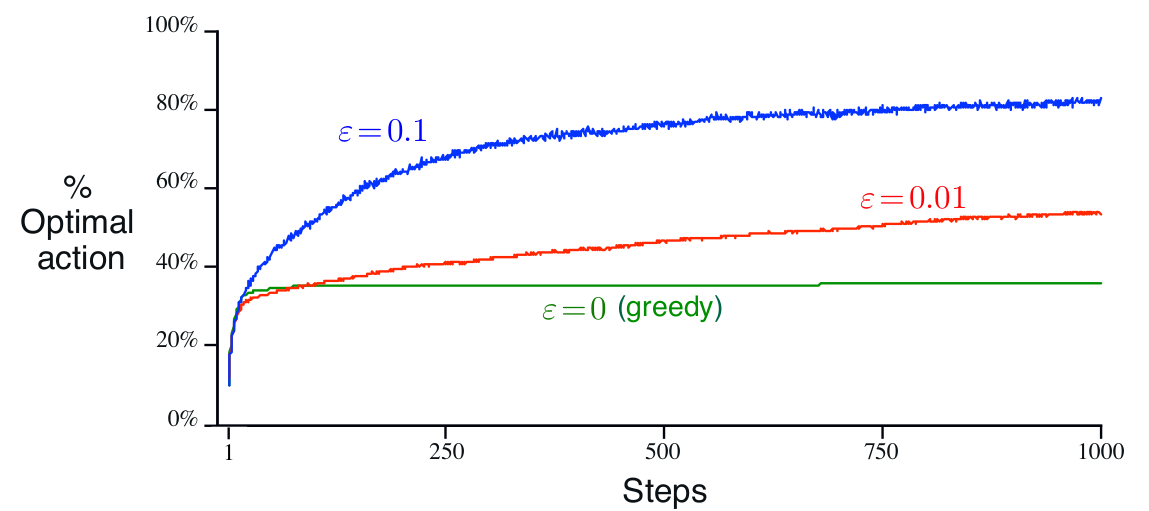
\includegraphics[scale=0.38]{images/eps_vs_optAction.png}
    \caption{Average performance of three agents using different $\epsilon$.  The data is averaged over 2000 runs.  Figure from \textit{Reinforcement Learning: An Introduction} by Sutton and Barto (2018).}
    \label{fig: eps_figure}
\end{figure}

During implementation, $\epsilon$ should decay out as $Q_t(a)$ approaches $q_*(a)$ to ensure knowledge of the agent is being adequately exploited. For non-stationary problems, $\epsilon$ should always be greater than zero to ensure other action values have not changed.

Algorithms to solve the \textit{k}-armed bandit problem are easily applied to situations where the concept of state is inert and only the actions are of concern;  a near impossibility in the real world.  

\subsubsection{Contextual Bandit}

A natural extension of the \textit{k}-armed bandit is associative search.  In associative search (sometimes called contextual bandit), different policies are associated with different situations \cite{bartosuttonbrouwer}.  Equation \ref{eq: state-action-value} is the extension of Equation \ref{eq: value} in the associative search problem.

\begin{equation}
    \centering
    q_*(x, u) = \mathbb{E}[R_t | X_t = x, U_t = u]
    \label{eq: state-action-value}
\end{equation}

Associative search is known as the method between \textit{k}-armed bandits and reinforcement learning.  In associative search, the objective is to associate optimal policies to different situations, but only maximizing the \textit{immediate} reward.  Often times, near term sacrifices are required to initiate the trajectory to a large lump sum reward at the terminal state.  For example, heavy capital and time investment is required for University in the short term.  However, the long term gain is so great that it outweighs the short term losses, making going to University an optimal policy for many individuals.

\subsubsection{The Reinforcement Learning Problem}

In order to find the true optimal policy (i.e., policy that returns the greatest rewards over a long time period), the topic of reinforcement learning is developed.  In reinforcement learning, sequential decision making is explored to identify the delayed reward signals from different actions and to ultimately find the optimal policy, $\pi^*$.  In the next sub-sections, the three fundamental reinforcement learning methods (Dynamic Programming, Monte Carlo, Temporal-Difference) will be introduced.

\subsection{Dynamic Programming Methods}
\subsubsection{Value-Iteration}
\subsubsection{Policy-Iteration}
\subsection{Monte Carlo Methods}
\subsection{Temporal-Difference Methods}
\subsection{Reinforcement Learning vs. Other "Learnings"}

Machine learning consists of the following four classes: i) Supervised learning, ii) Unsupervised learning, iii) Semi-supervised learning, iv) Reinforcement learning.  Supervised learning is fitting a model to a set of labeled data provided by a subject matter expert.  Subsequently, unsupervised learning is used on unlabeled data sets.  The objective of unsupervised learning is to explore the data and identify hidden features. Semi-supervised learning combines the strengths of supervised and unsupervised learning, and is especially useful \cite{machine_learning}.  Often times, industrial data will be partially labelled due to the time and cost associated with data labelling.  For supervised and unsupervised learning, only the labeled and unlabeled data can be used, respectively.  However, all data can be used in semi-supervised learning which allows for maximized data efficiency and increased model performance. Finally, reinforcement learning is a goal-directed learning from interactions with the environment \cite{sutton}.

Reinforcement learning is a unique class of machine learning.  An ideal supervised learning model can only be as good as the subject matter expert providing the labels to the data set, which may not be 100\%.  For example, in a complex control task, the control law is usually highly non-linear. Control experts can try to provide control strategies for such systems, but optimality may not be guaranteed for highly non-linear systems. Also, supervised learning is used to generalize responses for occurrences not present in the data \cite{sutton}.  Reinforcement learning works by directly interacting with the environment \textit{without labels}. Through adequate exploration, reinforcement learning will identify peculiar features to optimally control such problems [citation required].  Reinforcement learning is \textit{similar} to unsupervised learning in terms of identifying hidden structures within the environment.  However, reinforcement learning tries to maximize an internal scalar "reward" signal, rather than purely data mining.

Evolutionary methods, a family of optimization algorithms such as genetic algorithm, is most similar to reinforcement learning.  For a control problem, such methods can apply multiple static policies for different operating regimes \cite{sutton}.  Policy search is conducted by first initiating $k$ random input trajectories of length $N$, generating input matrix $\mathbb{U}_{[k, N]} \in \pi$.  Subsequently, the loss, $J_U$, of each $U$ is calculated based on the objective function.  Input trajectories with the lowest loss move onto the next generation and generates new pseudo-random input trajectories.  This process is repeated until optimal policy, $\pi^*$ is found for each operating regime \cite{ga_for_control}.

Evolutionary methods work well when the policy space is sufficiently small, easy to find, or a lot of time is available for optimization.  The biggest advantage of such methods compared to reinforcement learning is that the whole state does not need to be known.  However, such methods does not capture the reinforcement learning fundamentals of mapping $X \rightarrow U$.  Unlike evolutionary methods, reinforcement learning keeps memory of each indvidual interaction making it a more data efficient approach \cite{sutton}.

%%%%%%%%%%%%%%%%%%%%%%%%%%%%% End Section Intro to RL %%%%%%%%%%%%%%%%%%%%%%%%%%%%%%%%%%%%%%%


%%%%%%%%%%%%%%%%%%%%%%%%%%%%% Begin Section Tabular RL %%%%%%%%%%%%%%%%%%%%%%%%%%%%%%%%%%%%%%

\section{Tabular Q-learning}
\subsection{Introduction to Q-learning}
\subsubsection{Adaptation to Non-Stationary Problems}
\subsubsection{Incremental Implementation}
\subsubsection{Action Selection}
\subsubsection{Exploration in Tabular Q-learning}
\subsubsection{Reward Functions}
\subsubsection{Expected Returns for Different MDPs}

\subsection{Overall Setup}

%%%%%%%%%%%%%%%%%%%%%%%%%%%%% End Section Tabular RL %%%%%%%%%%%%%%%%%%%%%%%%%%%%%%%%%%%%%%%

%%%%%%%%%%%%%%%%%%%%%%% Begin Section Function Approximation %%%%%%%%%%%%%%%%%%%%%%%%%%%%%%%

\section{Function Approximation}
\subsection{Introduction to Function Approximations}
\subsection{Neural Network Basics}
\subsubsection{Neural Network Initialization}
\subsubsection{Gradient Descent Updating}
\subsubsection{Mini-batch Gradient Descent}
\subsubsection{Batch Normalization}
\subsubsection{Regularizations}

%%%%%%%%%%%%%%%%%%%%%%%%% End Section Function Approximation %%%%%%%%%%%%%%%%%%%%%%%%%%%%%%%


%%%%%%%%%%%%%%%%%%%%%%%%%%%%%%%%% Begin Section DDPG %%%%%%%%%%%%%%%%%%%%%%%%%%%%%%%%%%%%%%%

\section{Deep Deterministic Policy Gradient}
\subsection{Actor-Critic Intuition}
\subsection{Actor - Deterministic Policy Gradient}
\subsection{Critic - Deep Q-learning}

\newpage

\subsection{Exploration in DDPG}
\subsubsection{White Exploratory Noise}
\subsubsection{Ornstein-Uhlenbeck Exploratory Noise}
\subsection{Stabilization of Training}
\subsubsection{Experience Replay}
\subsubsection{Target Network}
\subsubsection{Adaptive Batch Gradient Descent}
\subsubsection{Reward Clipping}
\subsection{Input and State Constraints}
\subsection{Training Algorithm}

%%%%%%%%%%%%%%%%%%%%%%%%%%%%%%%%%% End Section DDPG %%%%%%%%%%%%%%%%%%%%%%%%%%%%%%%%%%%%%%%%


\chapter{Model Predictive Control}
\input{chapters/Chapter4:ModelPredictiveControl.tex}

\chapter{Comparison of RL and MPC}
\input{chapters/Chapter5:ComparisonofRLandMPC.tex}

\printbibliography

\end{document}